\documentclass[12 pt,a4paper]{article}\usepackage[]{graphicx}\usepackage[]{color}
% maxwidth is the original width if it is less than linewidth
% otherwise use linewidth (to make sure the graphics do not exceed the margin)
\makeatletter
\def\maxwidth{ %
  \ifdim\Gin@nat@width>\linewidth
    \linewidth
  \else
    \Gin@nat@width
  \fi
}
\makeatother

\definecolor{fgcolor}{rgb}{0.345, 0.345, 0.345}
\newcommand{\hlnum}[1]{\textcolor[rgb]{0.686,0.059,0.569}{#1}}%
\newcommand{\hlstr}[1]{\textcolor[rgb]{0.192,0.494,0.8}{#1}}%
\newcommand{\hlcom}[1]{\textcolor[rgb]{0.678,0.584,0.686}{\textit{#1}}}%
\newcommand{\hlopt}[1]{\textcolor[rgb]{0,0,0}{#1}}%
\newcommand{\hlstd}[1]{\textcolor[rgb]{0.345,0.345,0.345}{#1}}%
\newcommand{\hlkwa}[1]{\textcolor[rgb]{0.161,0.373,0.58}{\textbf{#1}}}%
\newcommand{\hlkwb}[1]{\textcolor[rgb]{0.69,0.353,0.396}{#1}}%
\newcommand{\hlkwc}[1]{\textcolor[rgb]{0.333,0.667,0.333}{#1}}%
\newcommand{\hlkwd}[1]{\textcolor[rgb]{0.737,0.353,0.396}{\textbf{#1}}}%
\let\hlipl\hlkwb

\usepackage{framed}
\makeatletter
\newenvironment{kframe}{%
 \def\at@end@of@kframe{}%
 \ifinner\ifhmode%
  \def\at@end@of@kframe{\end{minipage}}%
  \begin{minipage}{\columnwidth}%
 \fi\fi%
 \def\FrameCommand##1{\hskip\@totalleftmargin \hskip-\fboxsep
 \colorbox{shadecolor}{##1}\hskip-\fboxsep
     % There is no \\@totalrightmargin, so:
     \hskip-\linewidth \hskip-\@totalleftmargin \hskip\columnwidth}%
 \MakeFramed {\advance\hsize-\width
   \@totalleftmargin\z@ \linewidth\hsize
   \@setminipage}}%
 {\par\unskip\endMakeFramed%
 \at@end@of@kframe}
\makeatother

\definecolor{shadecolor}{rgb}{.97, .97, .97}
\definecolor{messagecolor}{rgb}{0, 0, 0}
\definecolor{warningcolor}{rgb}{1, 0, 1}
\definecolor{errorcolor}{rgb}{1, 0, 0}
\newenvironment{knitrout}{}{} % an empty environment to be redefined in TeX

\usepackage{alltt}
    \usepackage{xcolor}
    \definecolor{vertforet}{RGB}{153,202,67}
    \definecolor{vert}{RGB}{0,172,95}
    \definecolor{bleu}{RGB}{7,196,234}
    \definecolor{Orange}{RGB}{245,178,31}
    \definecolor{Rose}{RGB}{238,28,131}
    \definecolor{Gray}{RGB}{109,119,125}


    \usepackage{graphicx}
    \usepackage{pgf,tikz}
    \usetikzlibrary{shapes,arrows,chains,trees,calc,positioning}

    %-=-=-=-=-=-=-=-=
\IfFileExists{upquote.sty}{\usepackage{upquote}}{}
\begin{document}
    %-=-=-=-=-=-=-=-=

    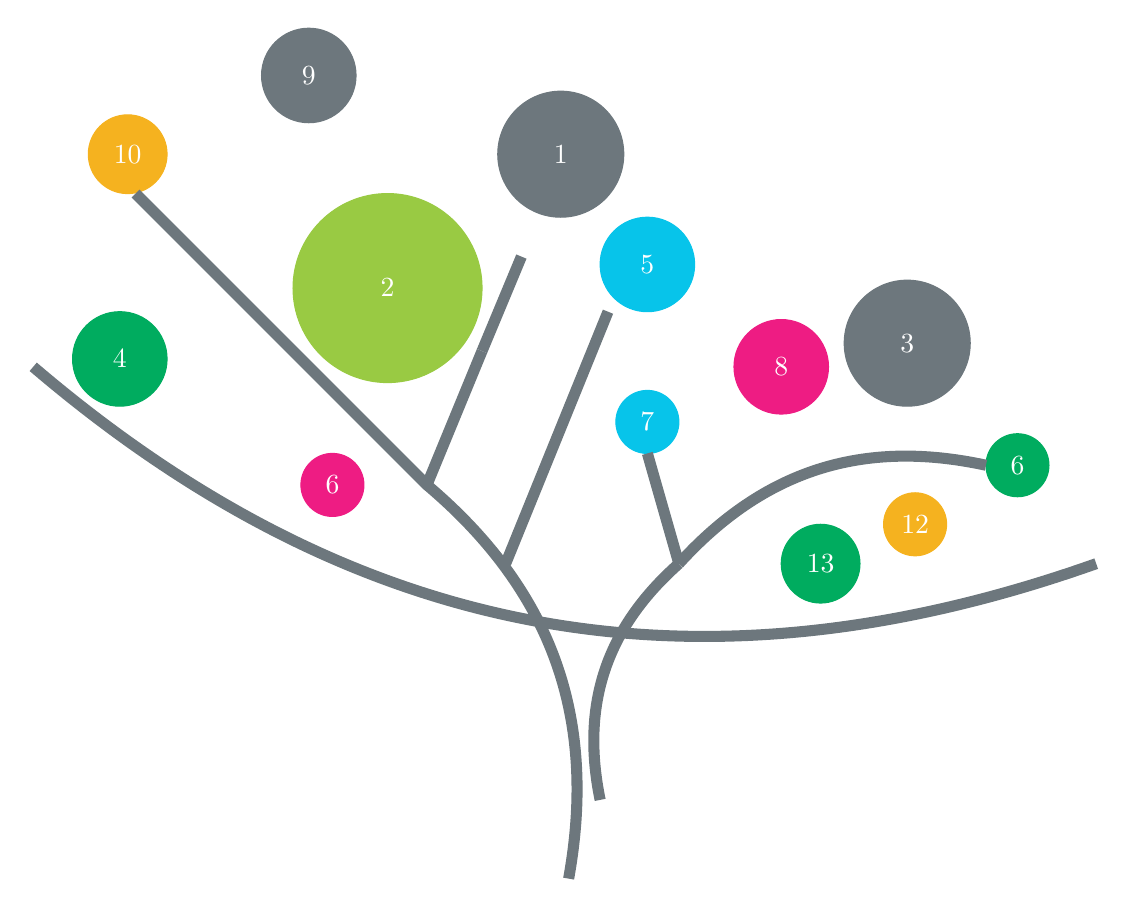
\begin{tikzpicture}[every node/.style={white}]
       \filldraw[Gray](0.2,3.7) circle(0.8) ;
    \node[white] at(0.2,3.7){1};
    \filldraw[vertforet](-2,2) circle(1.2)node{2} ;
    \filldraw[Gray](4.6,1.3) circle(0.8)node{3} ;
    \filldraw[vert](-5.4,1.1) circle(0.6) node{4};
    \filldraw[bleu](1.3,2.3) circle(0.6)node{5} ;
    \filldraw[Rose](-2.7,-0.5) circle(0.4) node{6};
    \filldraw[bleu](1.3,0.3) circle(0.4) node{7};
    \filldraw[Rose](3,1) circle(0.6)node{8};
    \filldraw[Gray](-3,4.7) circle(0.6) node{9};
    \filldraw[Orange](-5.3,3.7) circle(0.5) node{10};
    \filldraw[Rose](3.5,-1.5) circle(0.4) node{11};
    \filldraw[vert](6,-0.25) circle(0.4) node{6};
    \filldraw[Orange](4.7,-1) circle(0.4) node{12};
    \filldraw[vert](3.5,-1.5) circle(0.5) node{13};
    \path[draw=Gray,line width=4 pt](7,-1.5)to[bend left] (-6.5,1);
     \path[draw=Gray,line width=4 pt](0.3,-5.5)to[bend right] (-1.5,-0.5) to(-5.2,3.2);
    \path[draw=Gray,line width=4 pt] (-0.5,-1.5) to (0.8,1.7);
    \path[draw=Gray,line width =4 pt](-1.5,-0.5)--(-0.8,1.2);
    \path[draw=Gray,line width =4 pt](-0.8,1.2)--(-0.3,2.4);
    \path[draw=Gray,line width=4 pt] (0.7,-4.5) to[bend left] (1.7,-1.5);
\path[draw=Gray,line width=4 pt] (1.7,-1.5) to[bend left] (5.6,-0.25);
\path[draw=Gray,line width=4 pt] (1.7,-1.5) to(1.3,-.1);
    \end{tikzpicture}

    \end{document}
